% !TeX root = ../main.tex
% Add the above to each chapter to make compiling the PDF easier in some editors.

\chapter{Experimental Results}\label{chapter:results}

{\color{red} SOME INTRO SUMMARIZING THE FINDINGS IN BULLET POINTS}

We describe the complete experimental setups in Appendix \ref{appendix:experimental_setups}.

\section{Euclidean Flow Between Two Gaussians} \label{sec:gaussian_flow}

\begin{figure}[h!]
    \centering
    \begin{subfigure}{0.47\linewidth}
        \centering
        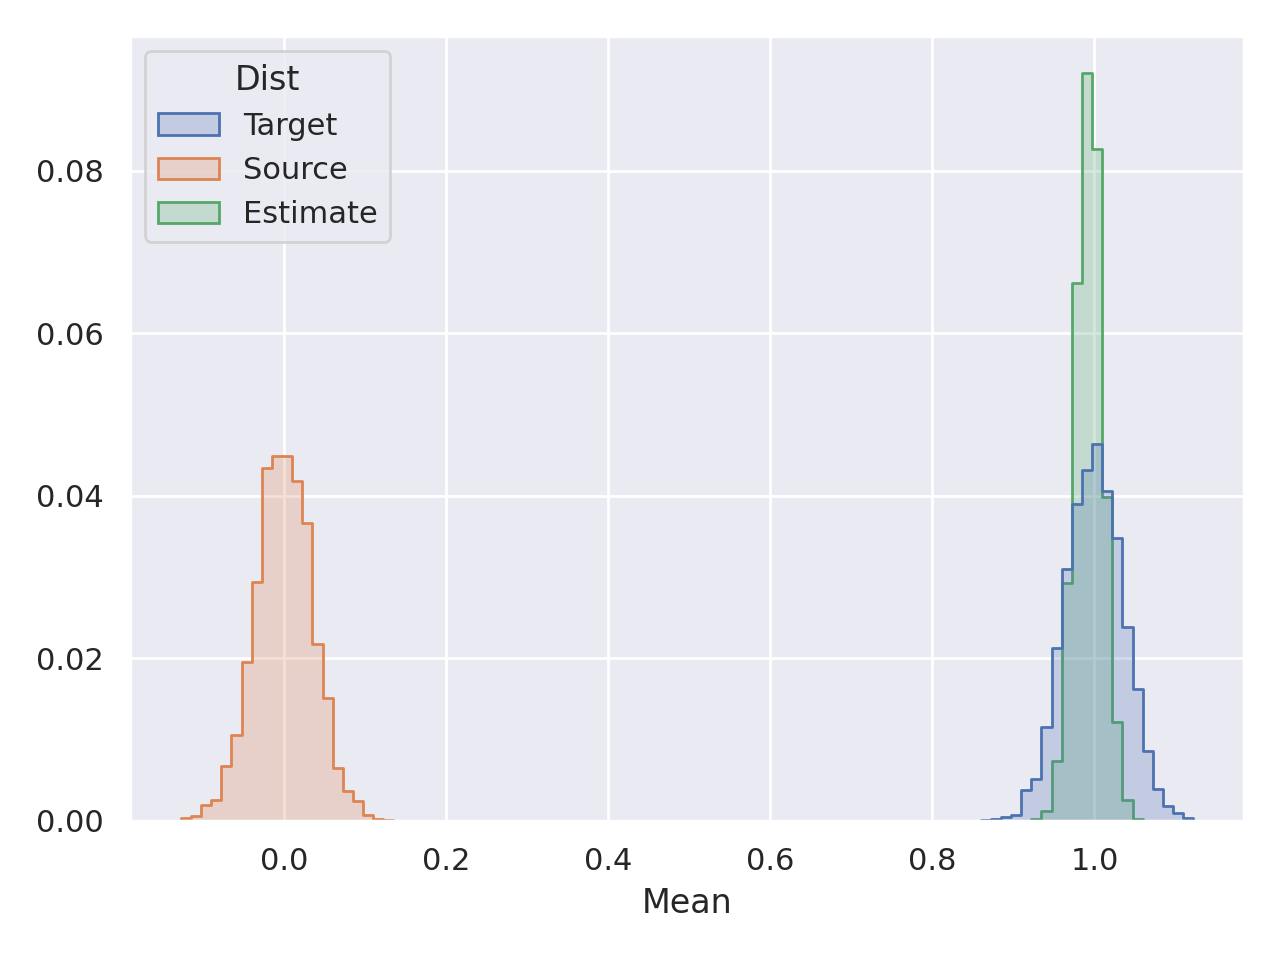
\includegraphics[width=\linewidth]{figures/gaussian/0.png}
        \caption{Deterministic sampling $(\varepsilon = 0)$}
        \label{fig:gaussian_deterministic}
    \end{subfigure}
    \begin{subfigure}{0.47\linewidth}
        \centering
        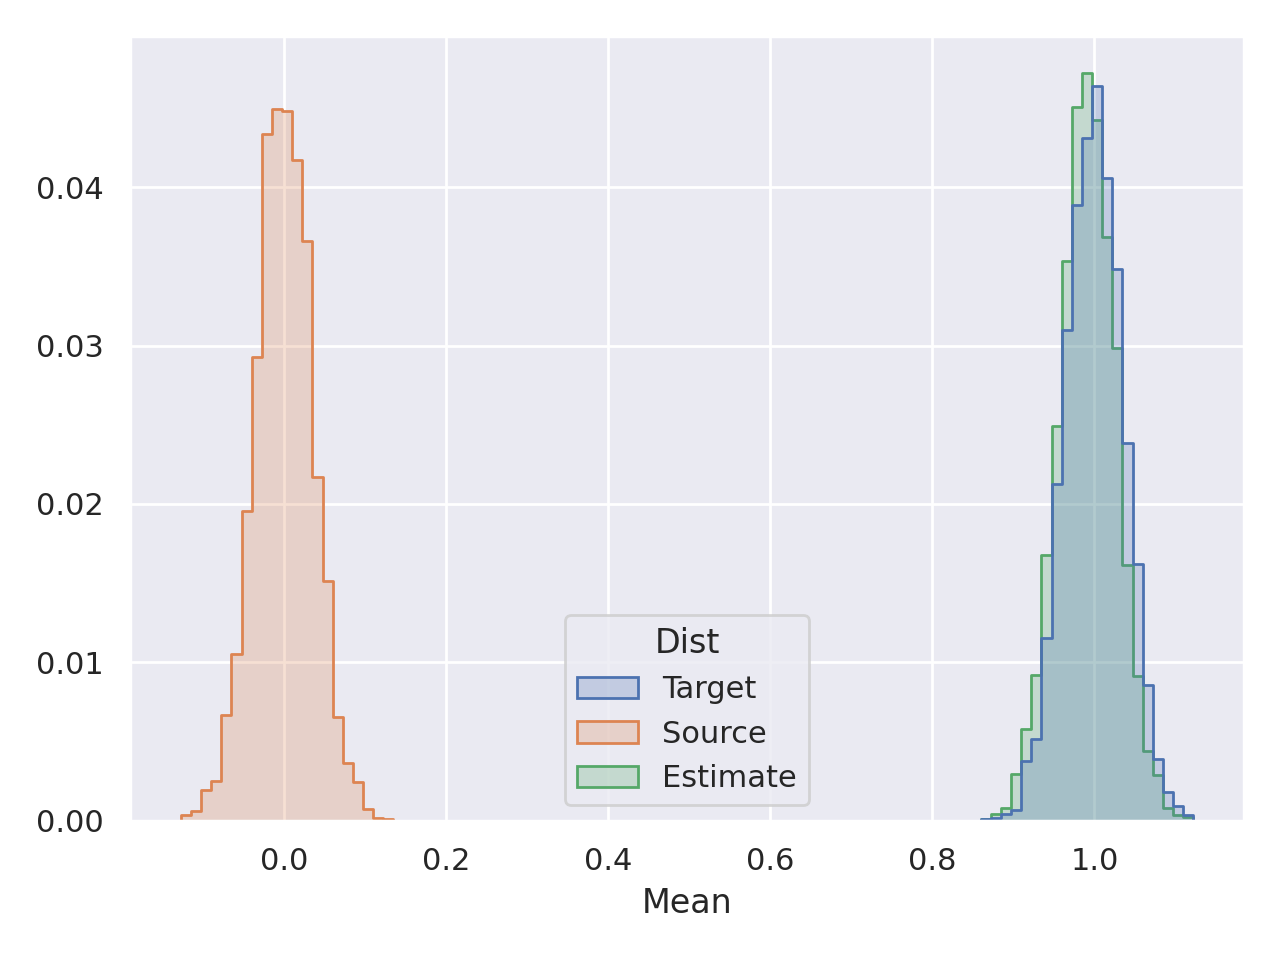
\includegraphics[width=\linewidth]{figures/gaussian/0.05.png}
        \caption{Stochastic sampling $(\varepsilon = 0.05)$}
        \label{fig:gaussian_stochastic}
    \end{subfigure}
    \caption{\label{fig:gaussian-results}\textbf{Histograms for the means of the weights generated by a Euclidean flow trained between two Gaussian distributions.} The flow fails to capture the variance in the target distribution with deterministic sampling, but this is corrected by stochastic sampling with $\varepsilon = 0.05$.} 
\end{figure}

To verify our approach of learning a flow model in weight-space, we begin our evaluation the toy task of learning a flow between two Gaussian distributions. The neural network is a small MLP with 30 input, two output dimensions, and two hidden layers of 16 neurons. We sample $X_0 \sim p_0 := \N(0, \mathbf{I})$ and $X_1 \sim p_1 := \N(1, \mathbf{I})$, and train our Euclidean flow to map $p_0$ to $p_1$ with independent coupling $q(x_0, x_1) = p_0(x_0)p_1(x_1)$. This is a relatively simpler task than learning over actual weights since each weight is sampled independently. 

Figure \ref{fig:gaussian-results} shows histograms of the means of the weights sampled from the flow with 100 Euler steps, and either deterministic or stochastic $(\varepsilon=0.05)$ sampling. Independent of the sampling method used, the flow covers the high-density center of the target distribution well, but the weights sampled deterministically fail to capture the variance in the target distribution. Stochastic sampling however appears to correct for this over-saturation and leads to more diverse samples. Overall, these results validates the feasability of learning a flow model in weight-space using graph neural networks, and we move on to tasks involving actual learned weights. 

\begin{figure}[t!]
    \centering
    \begin{subfigure}{0.47\linewidth}
        \centering
        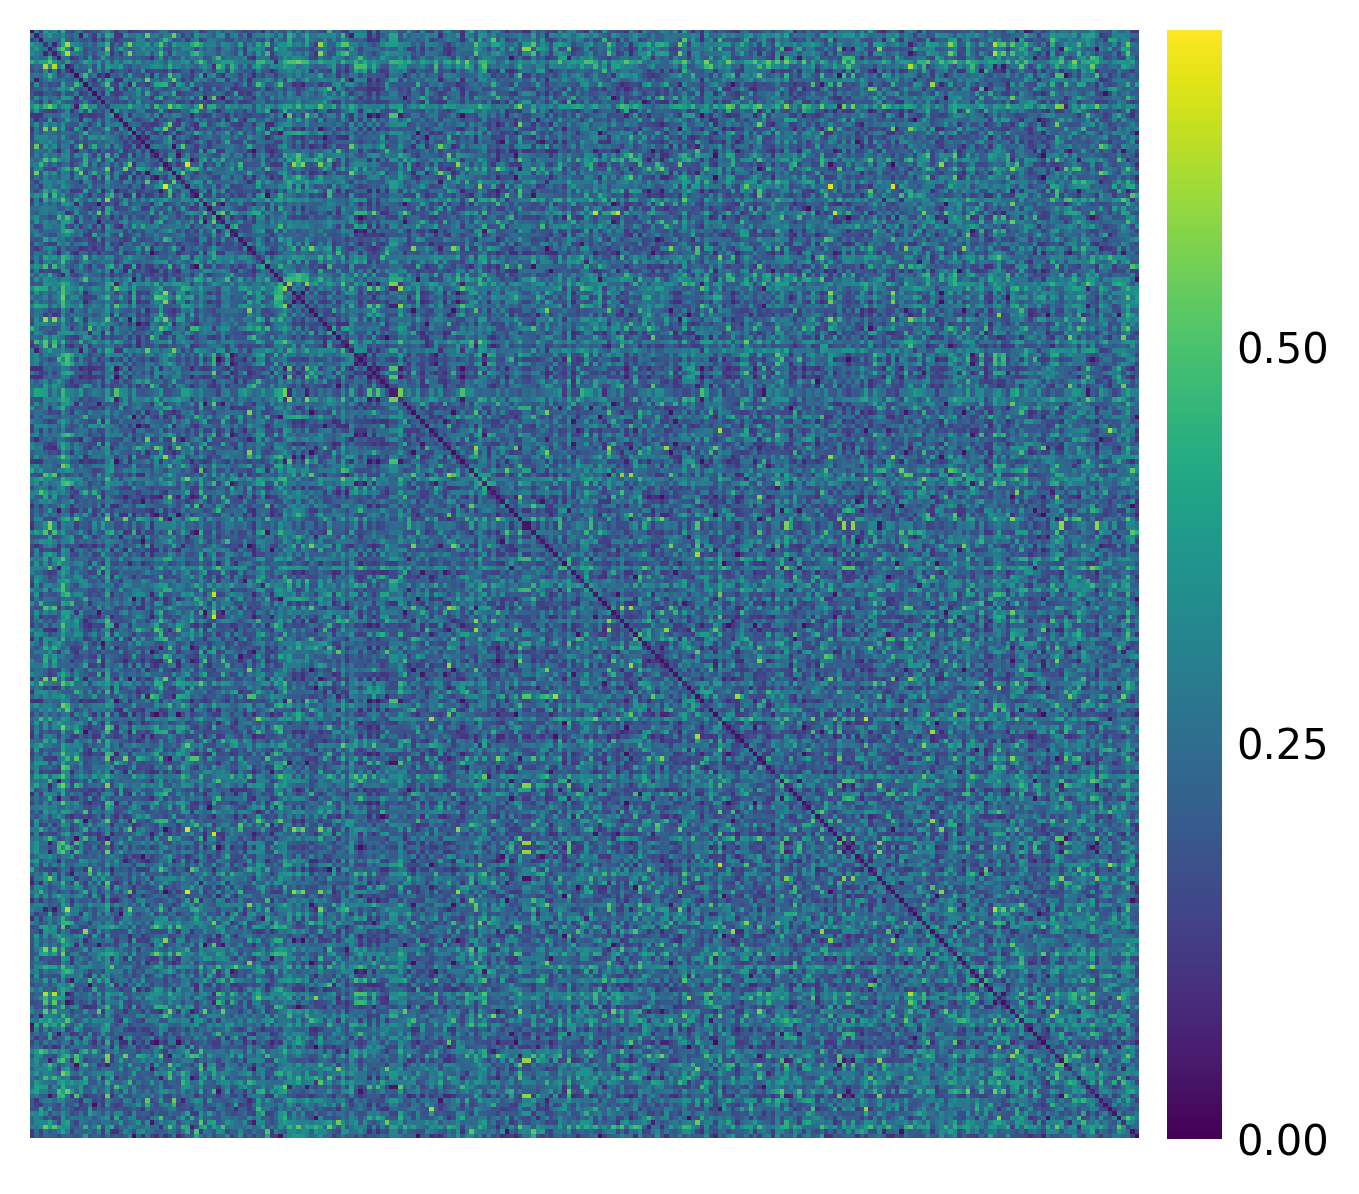
\includegraphics[width=\linewidth]{figures/uci_17/uci_17_unaligned.png}
        \caption{Unaligned (0.244 ± 0.009)}
        \label{fig:uci_unaligned}
    \end{subfigure}
    \begin{subfigure}{0.47\linewidth}
        \centering
        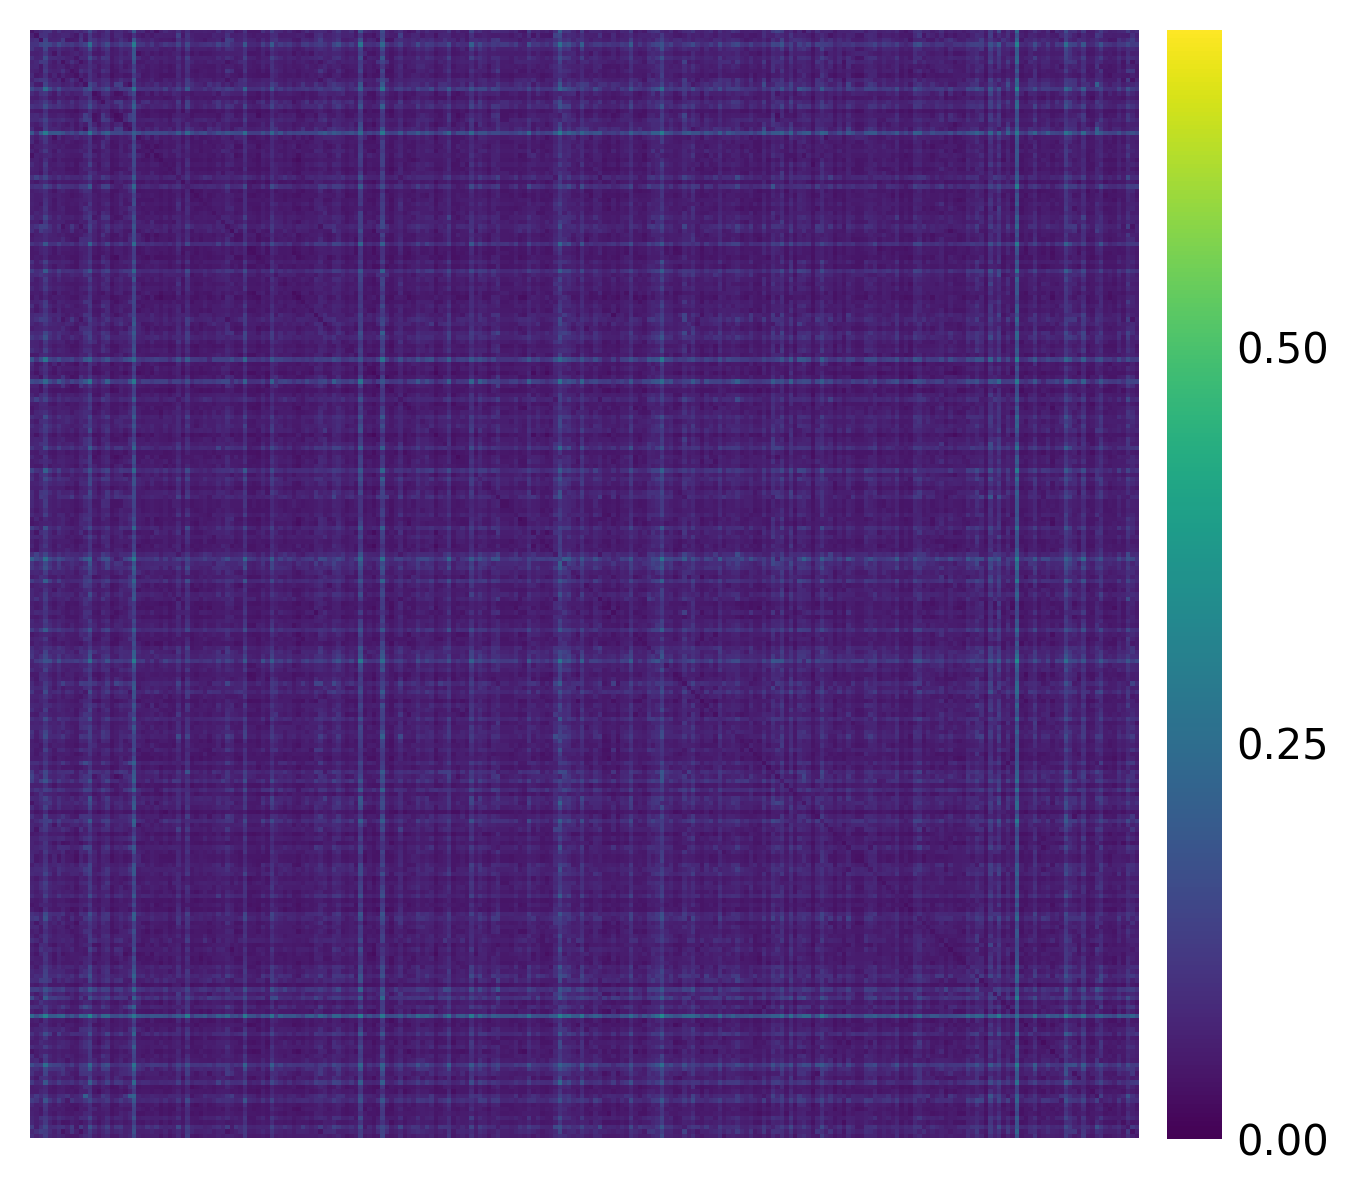
\includegraphics[width=\linewidth]{figures/uci_17/uci_17_aligned.png}
        \caption{Aligned (0.070 ± 0.001)}
        \label{fig:uci_aligned}
    \end{subfigure}
    \caption{\label{fig:uci_alignment}\textbf{Loss barriers for 250 weights across different optimization trajectories} (mean and standard deviations in parentheses) on the UCI Wisconsin Breast Cancer Diagnostics dataset. Aligning all weights to a single reference significantly reduces the loss barriers between the weights. } 
\end{figure}

\section{Classification with a Small Model} \label{sec:uci_classification}

\begin{table}[t!]
    \centering
    \begin{tabular}{lll}
        \toprule
        \textbf{Flow}  & \textbf{Accuracy} & \textbf{Loss} \\
        \midrule
        Euclidean                   & 0.998 ± 0.006     & 0.101 ± 0.05 \\ 
        Euclidean (aligned)         & 0.998 ± 0.006     & 0.070 ± 0.04 \\
        Euclidean (aligned + OT)    & 0.993 ± 0.010     & 0.053 ± 0.028 \\
        \midrule
        Normalized                  & 0.993 ± 0.009     & 0.027 ± 0.014 \\
        Normalized (aligned)        & 0.989 ± 0.011     & 0.030 ± 0.015 \\
        Normalized (aligned + OT)   & 0.988 ± 0.018	    & 0.044 ± 0.047 \\
        \midrule
        Geometric                   & 0.992 ± 0.011     & 0.019 ± 0.009 \\
        Geometric (aligned)         & 0.993 ± 0.001     & 0.018 ± 0.001 \\
        Geometric (aligned + OT)    & 0.991 ± 0.011 	& 0.020 ± 0.012 \\
        \midrule
        \textbf{Target}             & 0.992 ± 0.01      & 0.048 ± 0.032 \\
        \bottomrule
    \end{tabular}
    \caption{\label{tab:uci_class_table}\textbf{Test accuracy and loss ($\pm$ std) of the samples generated by flows with different design choices.} Euclidean and Normalized flows result in the most accurate weights, with Normalized flow generating lower-loss weights.}
\end{table}

After the toy Gaussian example, we move on to a relatively simple classification task to demonstrate that our flows can generate high-quality samples and compare the various design choices outlines in Chapter \ref{chapter:method}. The target model is an MLP with two hidden layers of 16 dimensions each and ReLU activations, on the binary classification task of the UCI Wisconsin Breast Cancer Diagnostic dataset \citep{streetNuclearFeatureExtraction1993}. We train all flows on the same dataset consisting of weights sampled from 100 independent trajectories optimized with Adam \citep{kingmaAdamMethodStochastic2017}. 

In addition to the availability of a large number of trained weights, this setup represents a preferable scenario in the sense that aligning all weights to a single reference eliminates the loss barriers between them to a large extent. Figure \ref{fig:uci_alignment} shows the pair-wise loss barriers (midpoint of the linear interpolation) before and after alignment for 250 randomly sampled weights from the set of Adam-optimized weights. The loss barriers are reduced considerably (from an average of 0.244 to 0.07) which supports the linear mode connectivity hypothesis for this setup. This should presumably make it easier to approximate the posterior distribution, as in the extreme case of zero-loss barriers between \textit{all} pairs of weights, the posterior would be convex. 

\textbf{Sample Quality.} Table \ref{tab:uci_class_table} compares the predictive quality of the samples generated by different flows with or without alignment and mini-batch OT couplings. All flows can generate samples with almost perfect accuracy, matching or exceedings (although ot significanly) the performance of Adam-optimized weights. Noticeably, the Geometric flow generates samples with lower loss than the Normalized flow, highlighting the benefit of modeling the vector field over the product geometry of normalized weights as well. Aligning all the weights to a reference before training, and training the flow with mini-batch OT couplings both decrease the loss of the generated samples for the Euclidean flow, but the same effect is not visible for the Normalized and Geometric flows. 

\begin{figure}[t!]
    \centering
    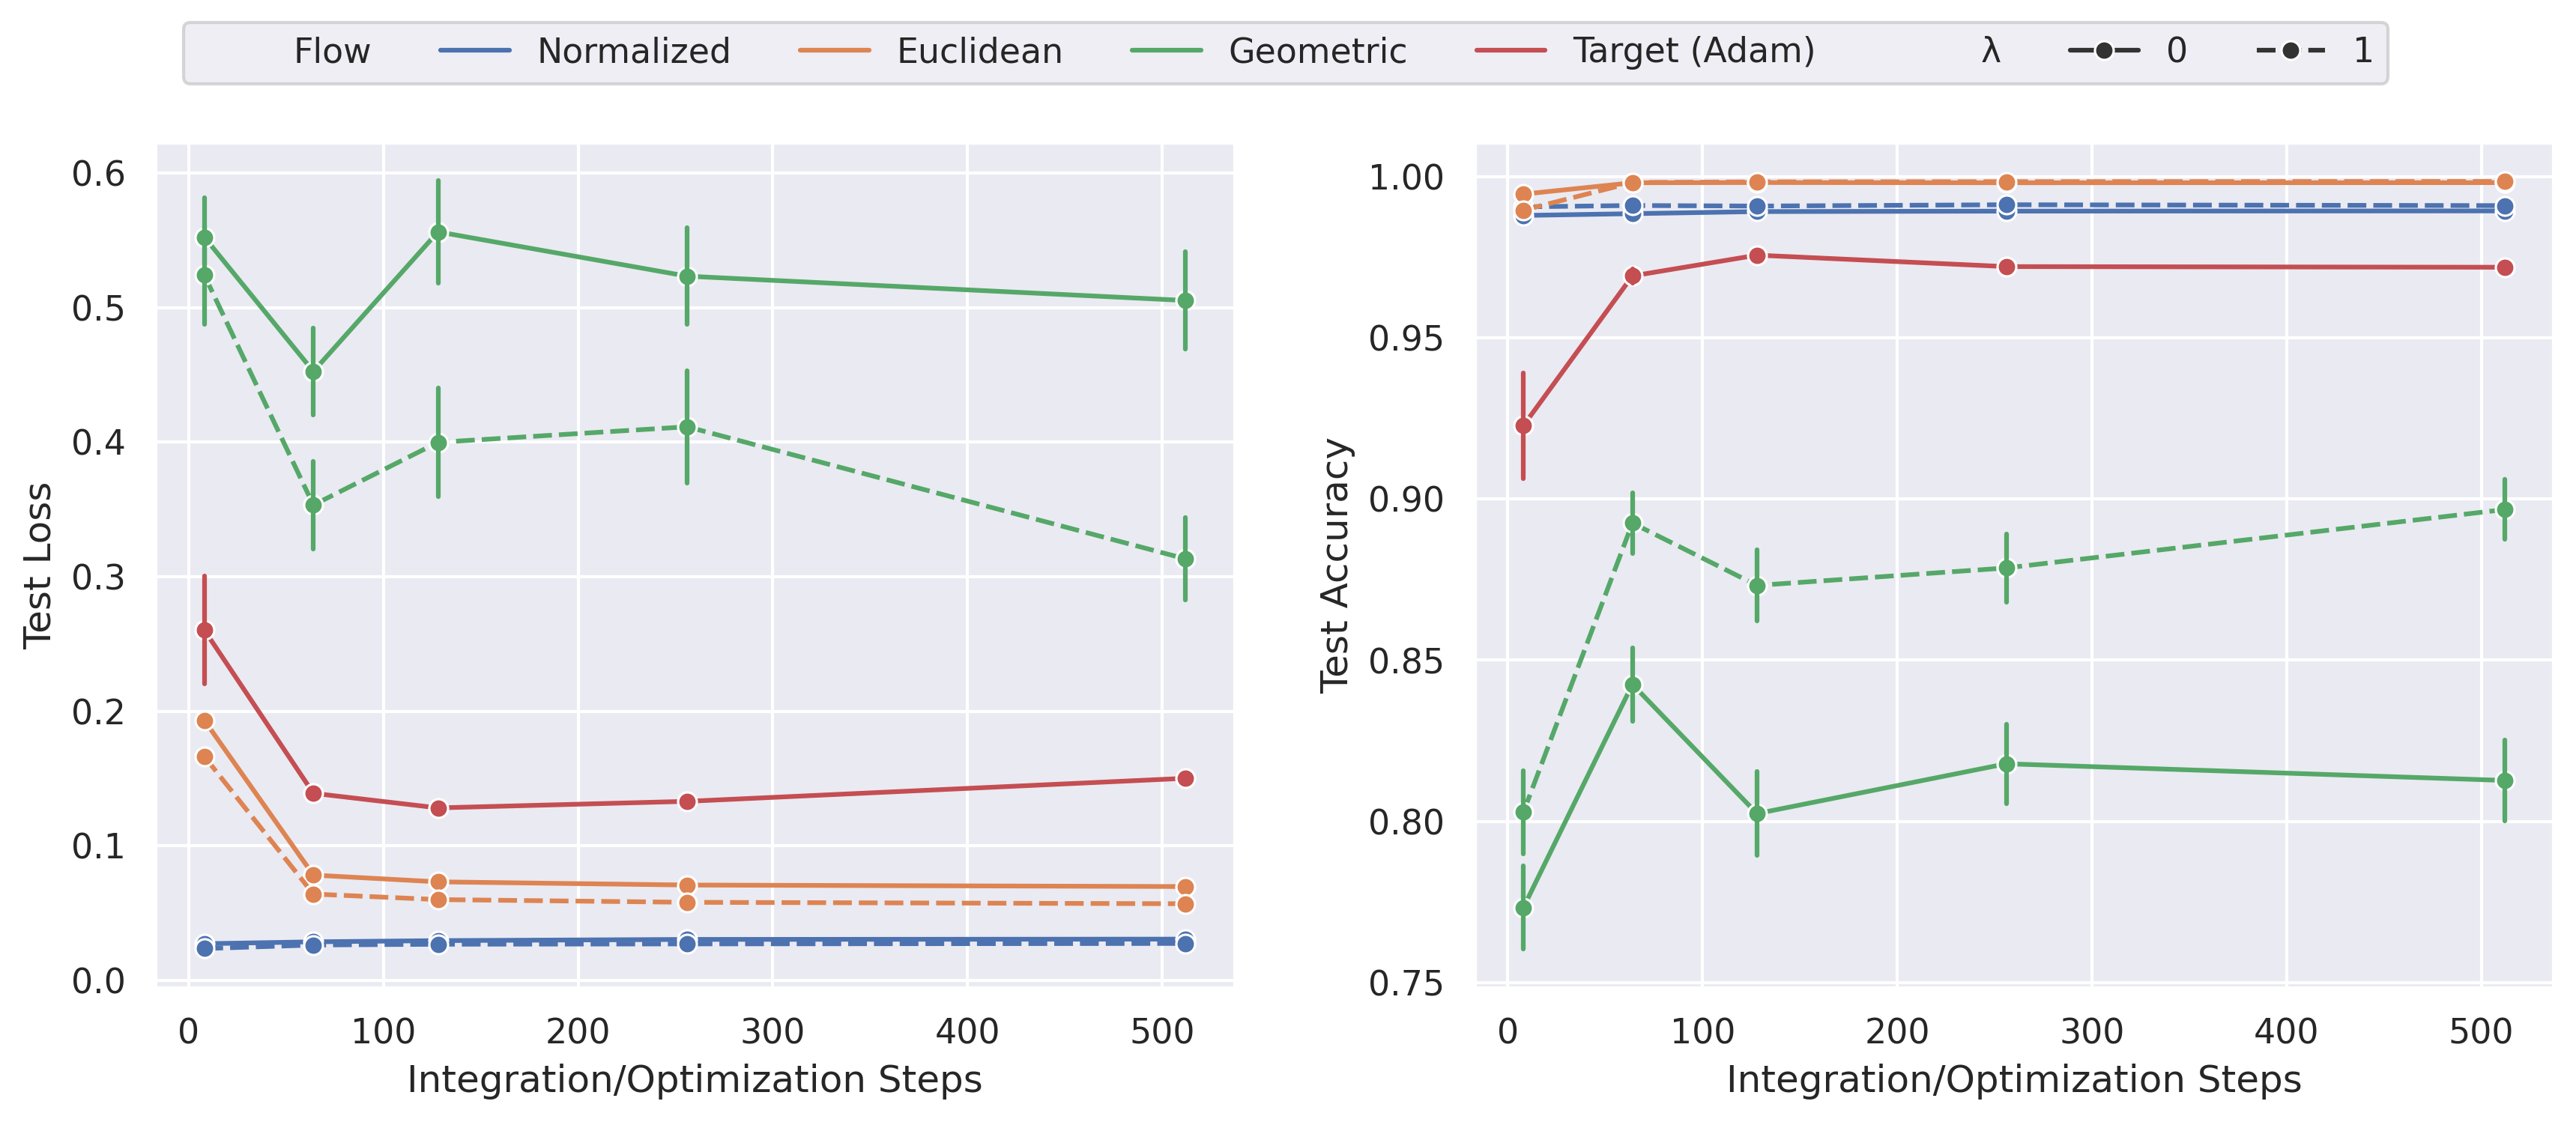
\includegraphics[width=\linewidth]{figures/uci_17/uci_17_steps_both.png}
    \caption{\label{fig:uci_steps}\textbf{Comparing the quality of the generated weights with Adam-optimized weights.} Weights generated by the Euclidean and Normalized flows have higher accuracy and lower loss than Adam-optimized weights, while the Geometric flow generated less accurate weights. Guidance during sampling improves sample quality.} 
\end{figure}

\textbf{Number of Integration Steps \& Guidance.} Figure \ref{fig:uci_steps} displays how the predictive performance of generated weights changes with the number of Euler steps performed to integrate the ODE. The main outcomes are:
\begin{itemize}
    \item Normalized and Geometric flows learn straighter paths compared to the Euclidean flow, apparent from the samples from the Euclidean flow showing a more significant improvement in quality going from 8 to 64 Euler steps. 
    \item For all three flows, guiding the integration with task gradients improves sample quality, but increasing the number of integration does not appear to significantly increase the effect of guidance. 
\end{itemize}


\section{MNIST Classification} \label{sec:mnist_classification}

We now move on to a harder classification task and larger models to evaluate different use cases of a weight-space flow. We start with the MNIST dataset, and an MLP with a single hidden layer of 10 neurons and ReLU activations, following the seutp used in \citep{peeblesLearningLearnGenerative2022}, but sample a smaller dataset along 20 independently initialized optimization trajectories.

This corresponds to a harder task than the UCI classification of the previous section for several reasons. The base MLP has around an order-of-magnitude of more parameters (7,960 rather than 802 parameters) while our GNN is in fact smaller. Moreover, the SGD/Adam-optimized weights do not reach perfect accuracy unlike in the UCI classification task. 

\begin{table}[t!]
    \centering
    \begin{tabular}{llll}
        \toprule
        \textbf{Flow}  & \textbf{Accuracy} & \textbf{Loss} & \textbf{Diversity} \\
        \midrule 
        Euclidean               & 0.737 ± 0.085	& 0.814 ± 0.286 & 0.00102 ± 0.00114 \\
        Euclidean (OT)          & 0.757 ± 0.077 & 0.753 ± 0.245 & 0.00085 ± 0.00094 \\
        \midrule
        Normalized              & 0.753 ± 0.074	& 1.537 ± 0.046 & 0.00086 ± 0.00055 \\
        Normalized (OT)         & 0.706 ± 0.078 & 1.608 ± 0.047 & 0.00117 ± 0.00074 \\
        \midrule
        Geometric               & 0.737 ± 0.070	& 1.457 ± 0.040 & 0.00073 ± 0.00049 \\
        Geometric (OT)          & 0.786 ± 0.064 & 1.443 ± 0.046 & 0.00093 ± 0.00063 \\
        \midrule
        \textbf{Target}         & 0.933 ± 0.009 & 0.231 ± 0.027 & 0.00002 ± 0.00001  \\
        \bottomrule
    \end{tabular}
    \caption{\label{tab:mnist_class_table}\textbf{Test accuracy, loss ($\pm$ std), and diversity of the samples generated by flows for classification on the MNIST dataset after alignment.} Geometric flow with OT couplings results in the beft-performing samples, but most flows are within one standard deviation of each other. }
\end{table}

\begin{figure}[t!]
    \centering
    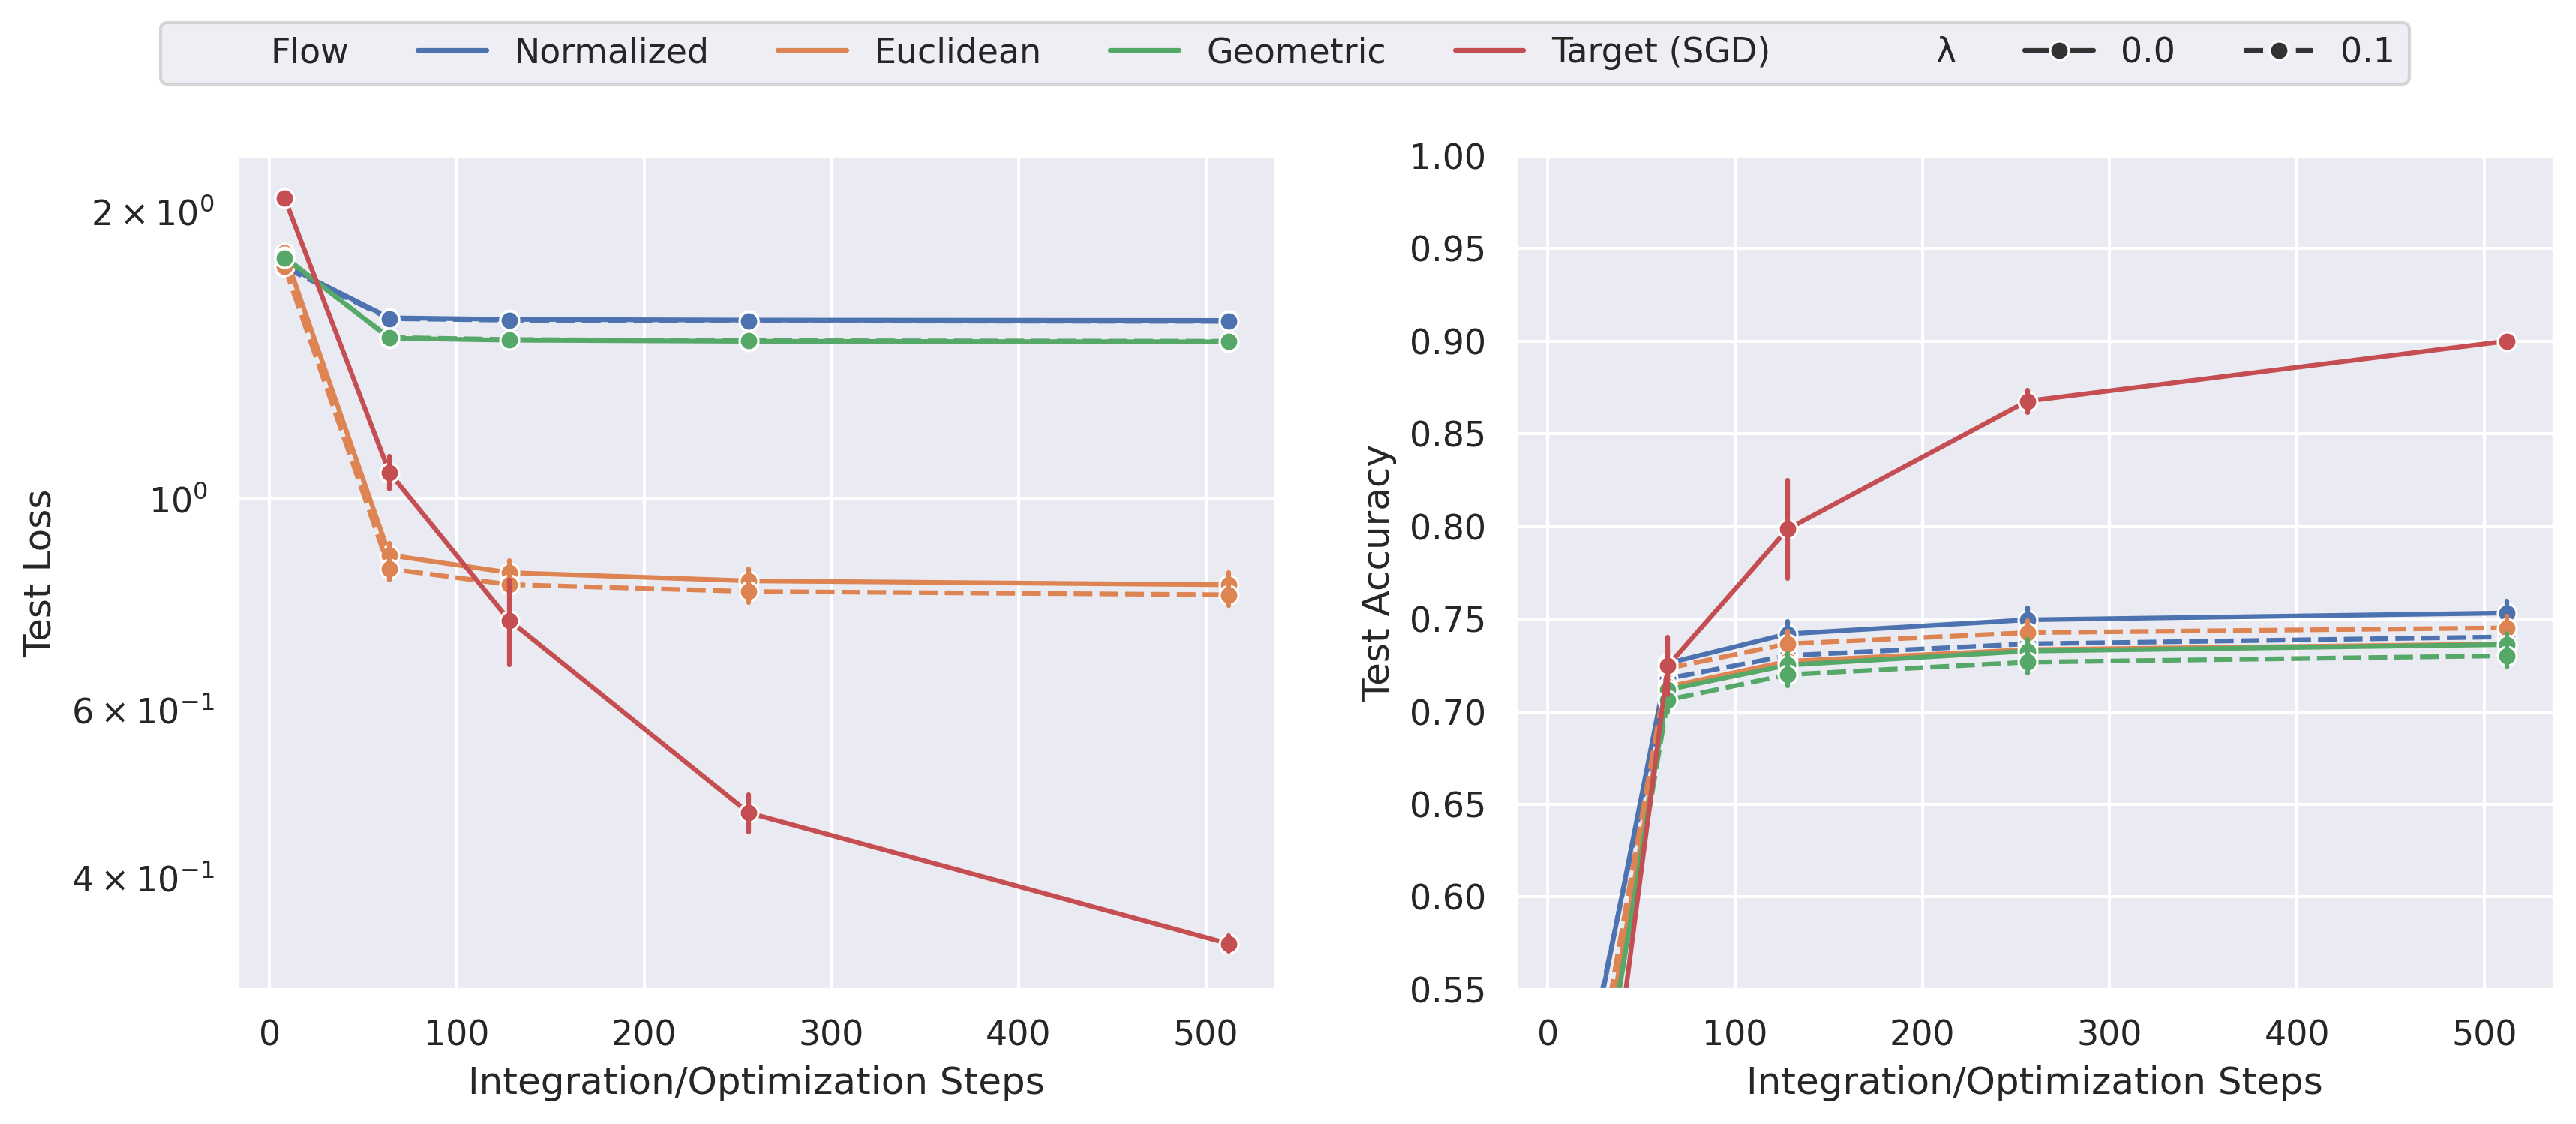
\includegraphics[width=\linewidth]{figures/mnist/mnist_steps_both.png}
    \caption{\label{fig:mnist_steps}\textbf{Comparing the quality of the generated weights with SGD-optimized weights.} After a very small number of steps, sampled weights are comparable in performance with SGD-optimized weights but plateau after around 64 steps. Geometric and Normalized flows again appear to lead to straighter paths.} 
\end{figure}


\subsection{Sample Quality and Diversity}

Table \ref{tab:mnist_class_table} shows the predictive performance and functional diversity of the weights generated by different kinds of flows trained on aligned weights. Functional diversity is a desirable property of a weight sampler, as more diverse weights could cancel each other's errors and make model averaging more effective. We focus on functional rather than parametric diversity since even if two neural networks do not have identical parameters, they could be computing the same function, and thus provide no benefit for model averaging. To measure the functional diversity in a set of neural networks, we compute the average pairwise Jensen-Shannon divergence (JSD) \citep{endresNewMetricProbability2003,mishtalJensenShannonDivergenceEnsembles2012} between the output (class probabilities) distributions of neural networks in the set. For a set of weights $S = \{ \theta_i \}_{i=1}^N$ and model $f$, we fix input points $\{ x_i \}_{i=1}^K$ and compute
\begin{equation} \label{eq:diversity}
    \text{Diversity}(S) := \frac{1}{N^2} \sum_{i, j} \text{JSD}\left(
        \{ f(\theta_i, x_l)\}_{l=1}^K, 
        \{f(\theta_j, x_l)\}_{l=1}^K
    \right)
\end{equation}
with JSD defined as 
\begin{equation}
    \text{JSD}(A, B) := 
    \frac{1}{2} \sum_{x \in A} p_A(x) \log \left( \frac{2p_A(x)}{p_A(x) + p_B(x)} \right) + 
    \frac{1}{2} \sum_{x \in B} p_B(x) \log \left( \frac{2p_B(x)}{p_A(x) + p_B(x)} \right)
\end{equation}
and we fit kernel density estimators to both sets to estimate the densities $p_A$ and $p_B$. 

Table \ref{tab:mnist_class_table} displays the test accuracy, loss, and diversity (Equation \ref{eq:diversity}) of the samples generated with each flow, trained after alignment, and with independent as well as mini-batch OT couplings. While the accuracy of sampled weights are generally within one standard deviation of each other, the Geometric flow with OT couplings results in the highest accuracy. However, unlike the previous UCI classification task, the sampled weights individually perform worse than SGD-optimized weights. 

The output distributions of the generated weights shows higher diversity than SGD-optimized weights, although this is also influenced by the generated weights performing worse. Nevertheless, as we will observe in the next chapter, this diversity makes model averaging more effective and considerably increases the predictive performance of generated weights. 

Figure \ref{fig:mnist_steps} shows how sample quality varies with the number of steps for our three flows trained with independent couplings, and sampled with and without guidance. Unlike the previous task where the sampled weights were directly of almost perfect accuracy, the sample quality for MNIST flows plateau after a certain number of steps, and SGD-optimized weights show superior performance. Similar to the results on the UCI classification task, Normalized and Geometric flows also show less improvement with a larger number of steps, indicating that the flows have learned straighter paths then the Euclidean flow. 

\subsection{Posterior Predictive}

\begin{figure}[t!]
    \centering
    \begin{subfigure}{0.55\linewidth}
        \centering
        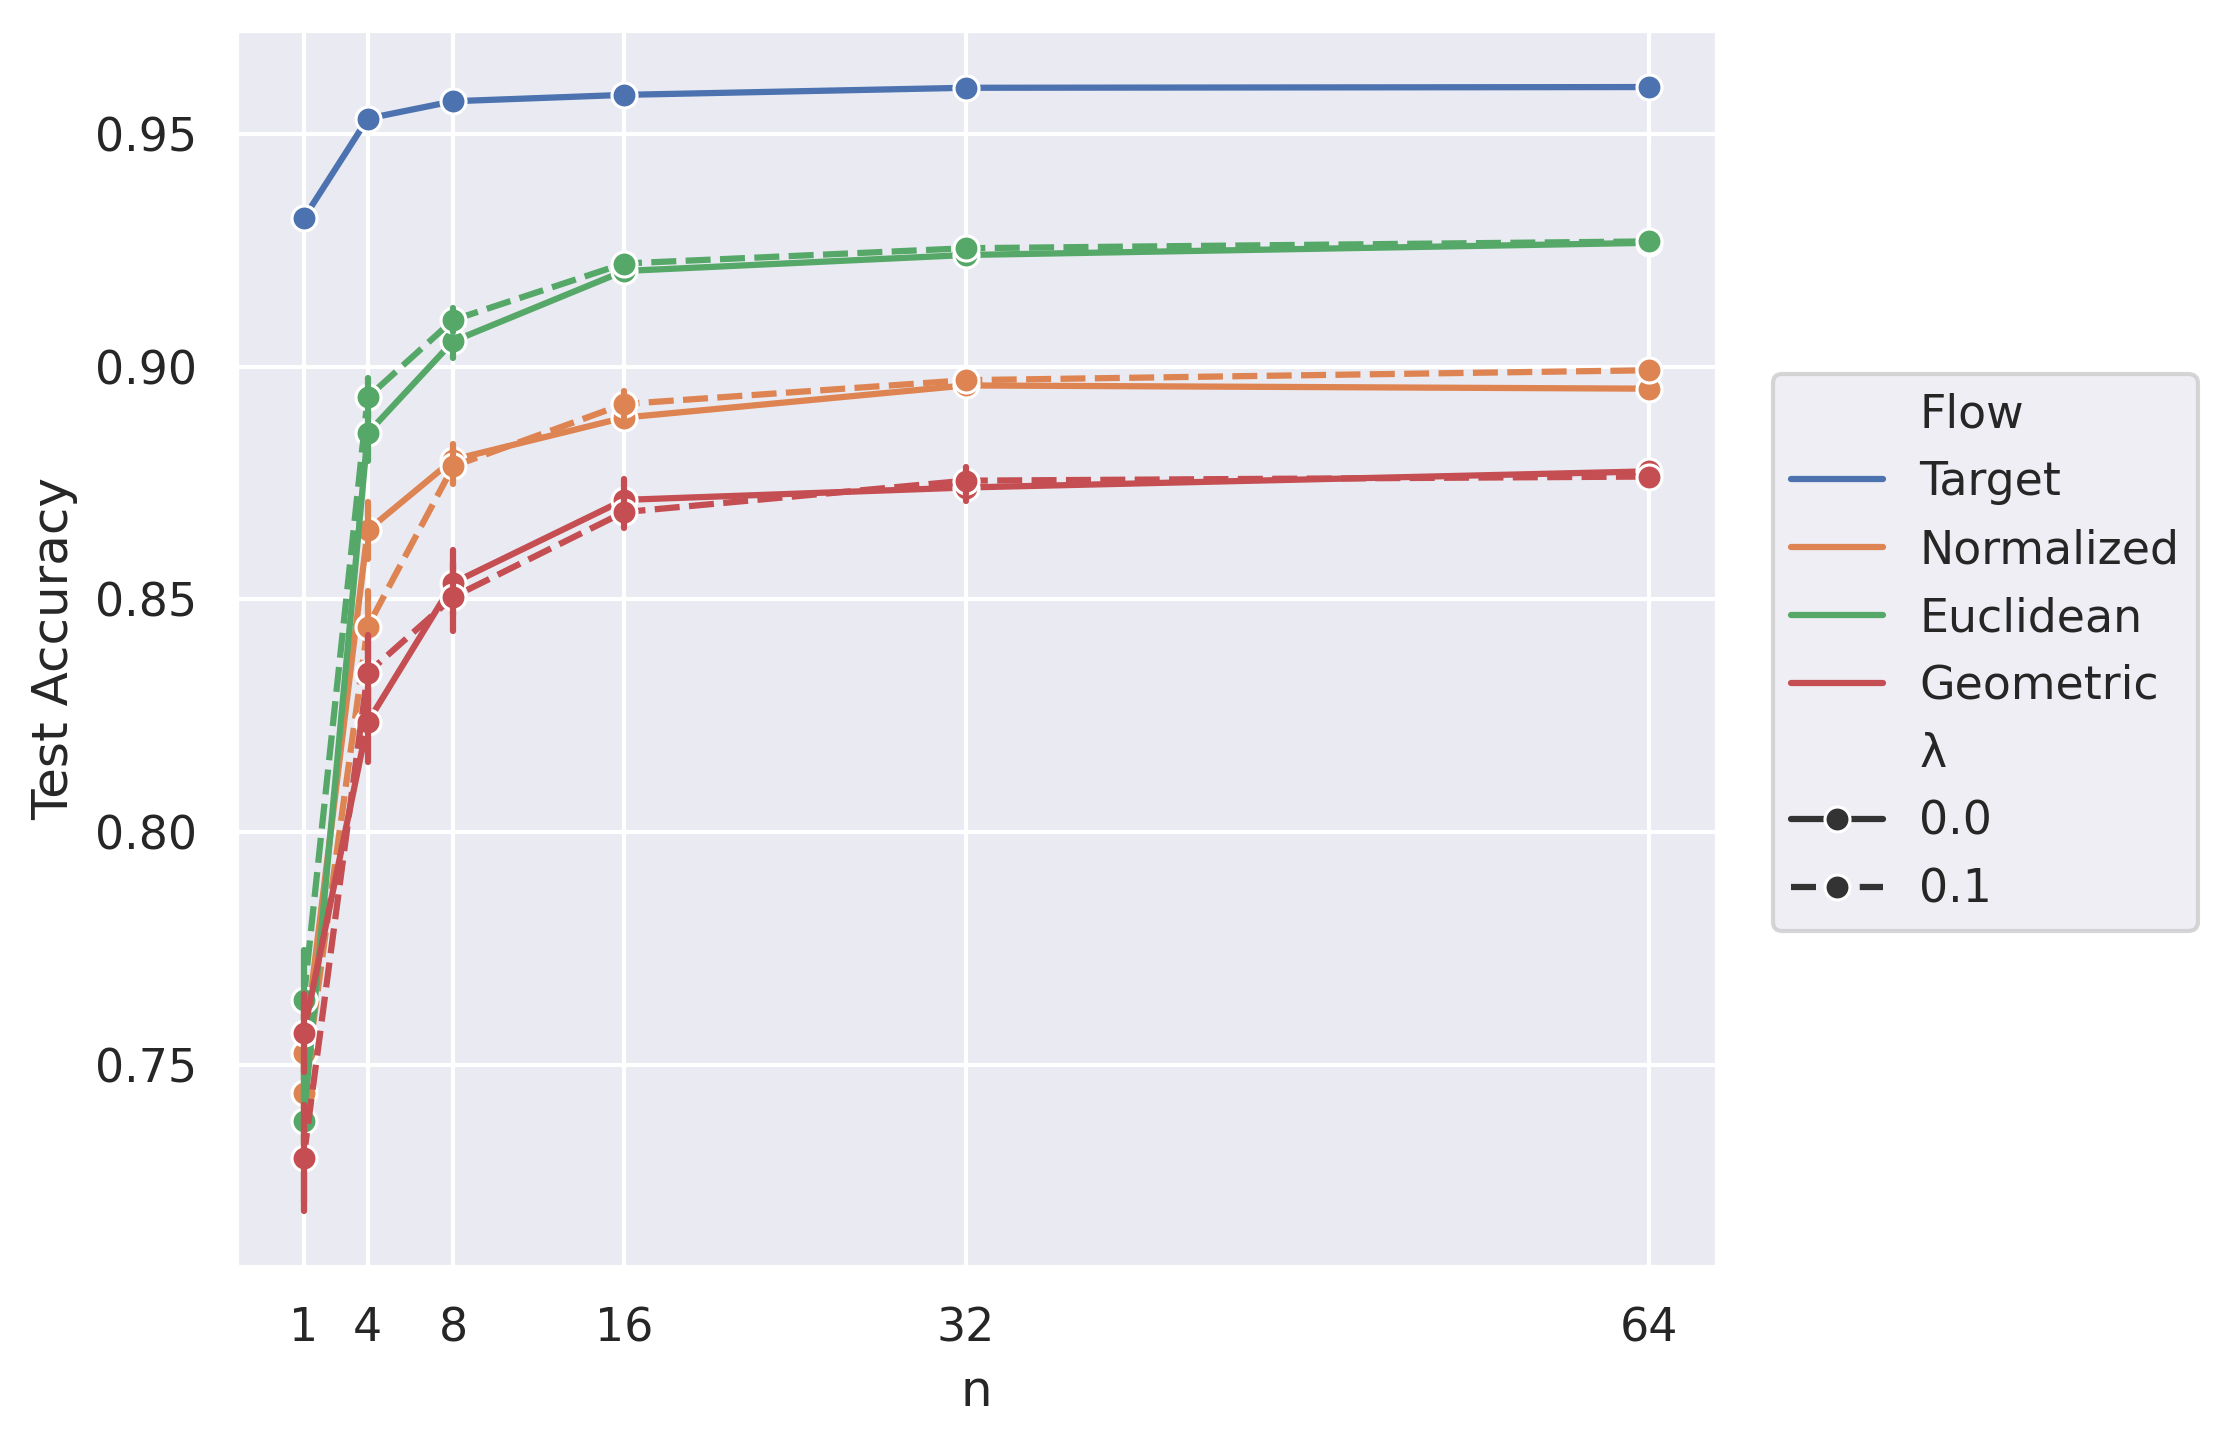
\includegraphics[width=\linewidth]{figures/mnist/mnist_model_averaging.png}
        \caption{Independent Couplings}
    \end{subfigure}
    \begin{subfigure}{0.43\linewidth}
        \centering
        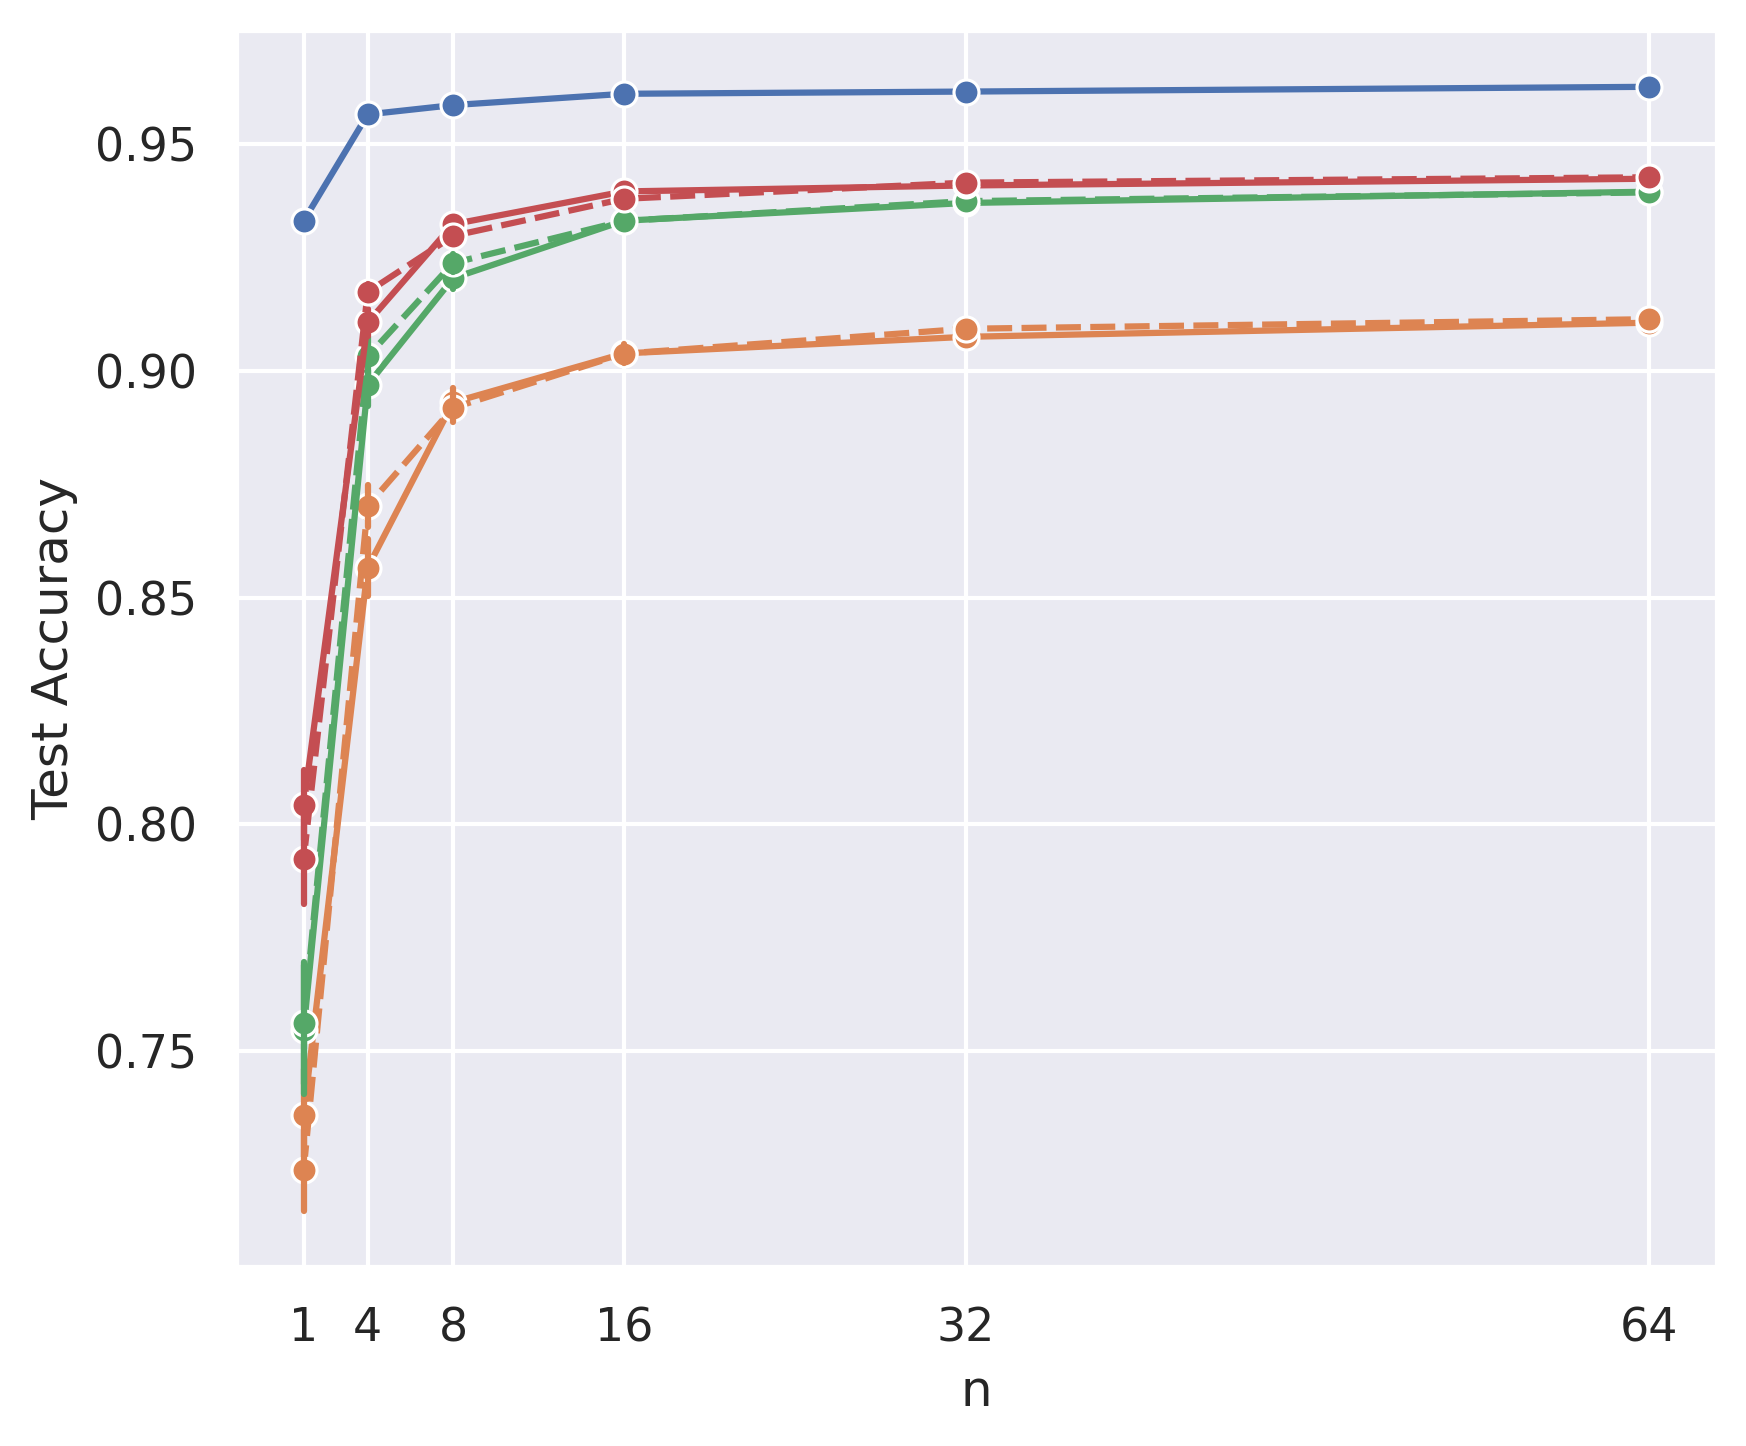
\includegraphics[width=\linewidth]{figures/mnist/mnist_model_averaging_OT.png}
        \caption{OT Couplings}
    \end{subfigure}
    % 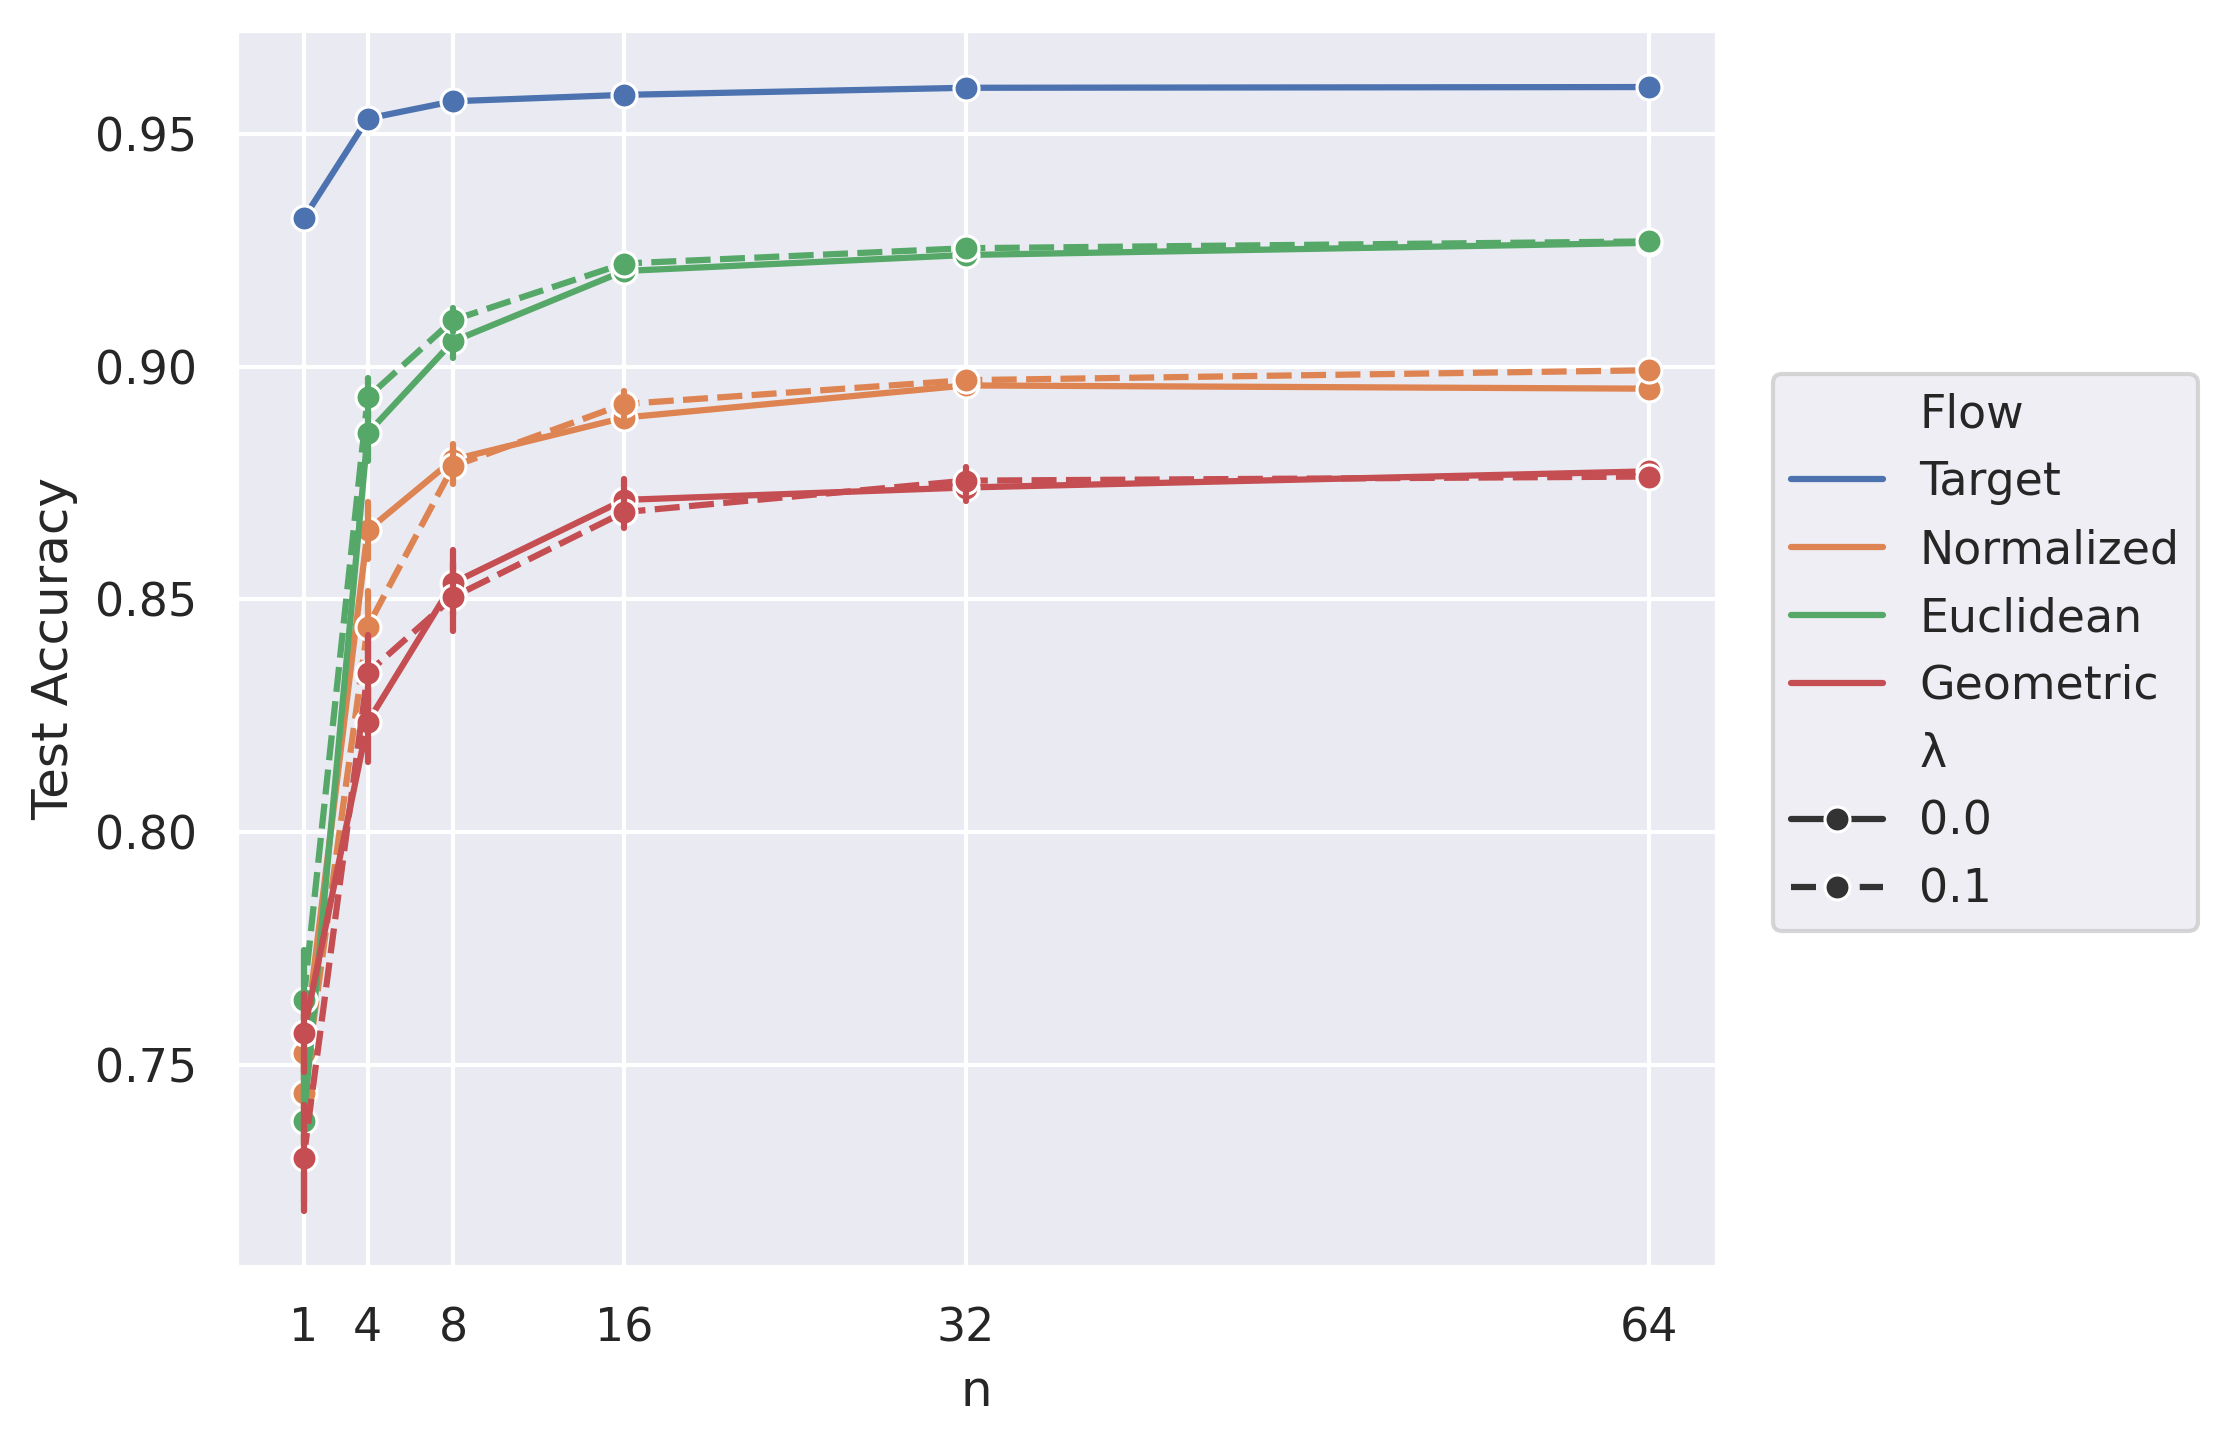
\includegraphics[width=0.7\linewidth]{figures/mnist/mnist_model_averaging.png}
    \caption{\label{fig:mnist_averaging}\textbf{Accuracy of the predictions averaged over various numbers of samples from the flows' pushforward distributions, comparing independent and OT couplings.} The Euclidean flow shows the highest accuracy, reaching the accuracy of individual SGD-optimized weights.} 
\end{figure}

We now evaluate the predictive performance of the sampled weights after Bayesian model averaging; i.e. for each flow, we sample from its pushforward distribution $\hat p_1 (\theta)$ and compute a Monte Carlo estimate for the expectation $\bbE_{\hat p_1 (\theta)} \left[ p(y\vert x, \theta) \right]$, as in Equation \ref{eq:model_averaging}. Figure \ref{fig:mnist_averaging} displays the accuracy of predictions averaged over increasing numbers of samples from $\hat p_1$, comparing our three flows as well as independent and mini-batch OT couplings. With independent couplings, the Euclidean flow results in the highest acuracies, noticeably reaching the accuracy of individual SGD-optimized weights. 

Training the flows with OT couplings improves the predictive performance of all three after model averaging. The improvement for the Geometric flow is more significant than that of the Euclidean and Normalized flows, moving from $\sim87\%$ to $~94\%$. This supports the results in Table \ref{tab:mnist_class_table} that the Geometric flow benefits the most from OT couplings. 

\section{Transferability to Other Tasks} \label{sec:task_generalization}

\begin{table}[t!]
    \centering
    \begin{tabular}{lll}
        \toprule
        \textbf{Flow} & \textbf{Accuracy} & \textbf{Loss} \\
        \midrule
        \textbf{Adam-optimized} & 0.908 ± 0.003 & 0.334 ± 0.008 \\
        \midrule
        \textbf{With Guidance} & & \\
        Euclidean   & 0.754 ± 0.082     & 0.764 ± 0.252 \\
        Normalized  & 0.724 ± 0.081     & 1.543 ± 0.045 \\
        Geometric   & 0.730 ± 0.067     & 1.470 ± 0.043 \\
        \midrule
        \textbf{No guidance} & 0.080 ± 0.030 & 9.601 ± 1.402 \\ 
        \bottomrule
    \end{tabular}
    \caption{\label{tab:mnist_generalization}\textbf{Predictive performance of samples from the MNIST flows with guidance ($\lambda = 0.1$) from Fashion-MNIST task gradients.} Although the base model (Adam) accuracy is lower than for MNIST, samples obtained with guidance reach an accuracy similar to that of the samples obtained without guidance on MNIST, indicating that a flow trained on one dataset can be transferred to another dataset via guidance. }
\end{table}


As a potential use case of our flows, we now evaluate the effectiveness of a flow trained on weights from a dataset (e.g. MNIST) different than the target dataset (e.g. Fashion-MNIST) using the same architecture, although the GNNs we model our flow with can be applied to architectures other than the one they were trained on. There are three main ways we can evaluate this performance:
\begin{enumerate}
    \item Evaluate the samples directly.
    \item Guide sampling with gradients from the target task. 
    \item Initialize model with sampled weights and train on the target dataset.
\end{enumerate}

First, Table \ref{tab:mnist_generalization} shows the performance (on Fashion-MNIST) of samples from flows trained with MNIST weights but sampled with guidance from the Fashion-MNIST task gradients over 512 Euler steps. First, expectedly, the last row of the table shows that samples obtained directly from the MNIST flows without guidance achieve an average accuracy of 8\%, which is not better than random guessing. However, although the accuracy of the base model after optimization with Adam is slighly lower for Fashion-MNIST compared to MNIST, samples from all three flows achieve a test accuracy of at least 72\%, which is similar performance of the samples obtained without guidance from the same flows on MNIST. 

These results highlight that even though the flows are trained on weights obtained over one dataset, they can capture some salient features shared across optimization landscapes, and can be adapted to different datasets without having to train them from scratch, in this case only by guiding the sampling process with task gradients which is significantly cheaper than training the entire flow from scratch.  

Next, we evaluate if the samples from the MNIST flows obtained without any guidance provide a more effective initialization scheme then random initialization. 

\begin{figure}[h!]
    \centering
    \begin{subfigure}{0.47\linewidth}
        \centering
        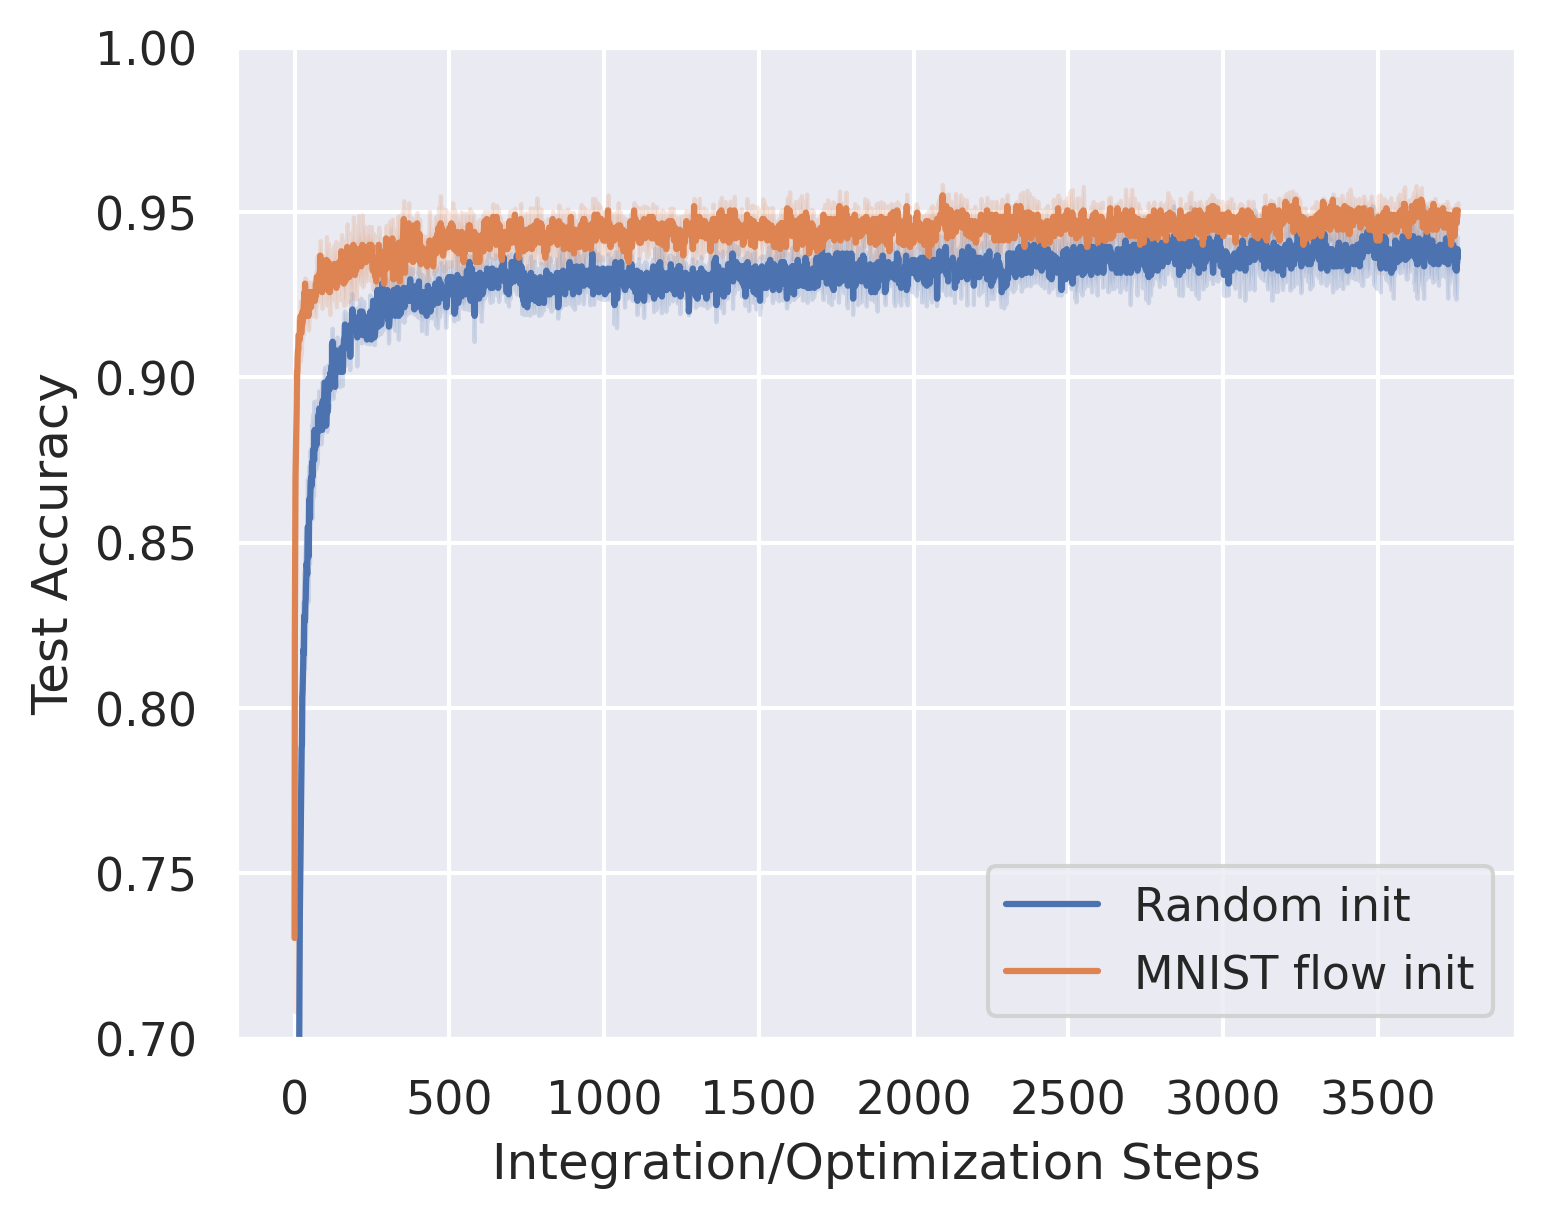
\includegraphics[width=\linewidth]{figures/mnist/mnist_init_acc.png}
        \caption{Test Accuracy}
    \end{subfigure}
    \begin{subfigure}{0.47\linewidth}
        \centering
        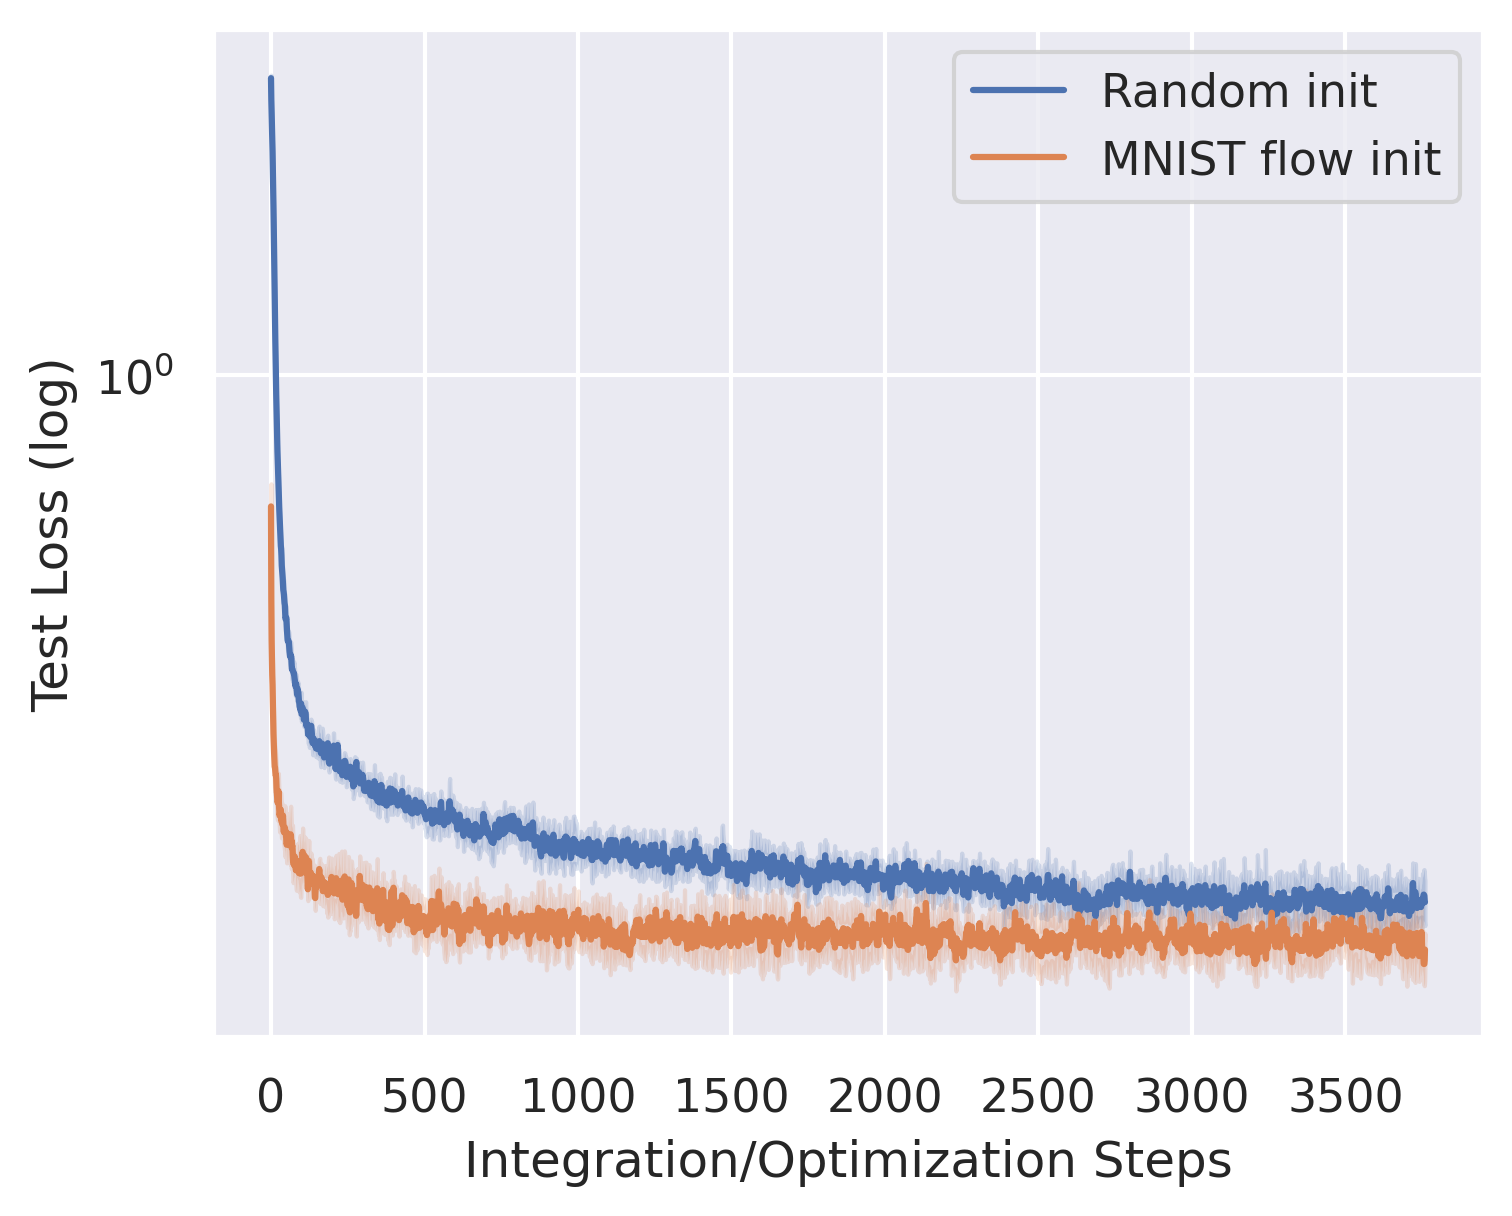
\includegraphics[width=\linewidth]{figures/mnist/mnist_init_loss.png}
        \caption{Test Loss}
    \end{subfigure}
    \caption{\label{fig:mnist_init}\textbf{Optimization trajectories of Adam on Fashion-MNIST with initial weights sampled from an isotropic Gaussian and the Euclidean flow trained on MNIST weights.} } 
\end{figure}

{\color{red} EXPLAIN}


